\section{问题一求解与分析}
\subsection{问题的描述与分析}

场景 A 把每个子图作为独立 Task。即使两个相邻 Task 被安排到同一核心，前一 Task 的私有缓存也不再可用；跨子图张量须由 DDR 中转。同核顺序和跨核前驱分别触发不同的固定等待，因此切图粒度本身会改变调度开销。过粗的子图压缩并行度，过细的子图增加 Task 切换及搬运。图~\ref{fig:q1-overview} 将计算图、依赖约束、候选切图及官方核验放在一条研究链中，具体统计图在本章结果段给出。

% Generated figure only; description and reference belong before this input.
\begin{figure}[!htbp]
\centering
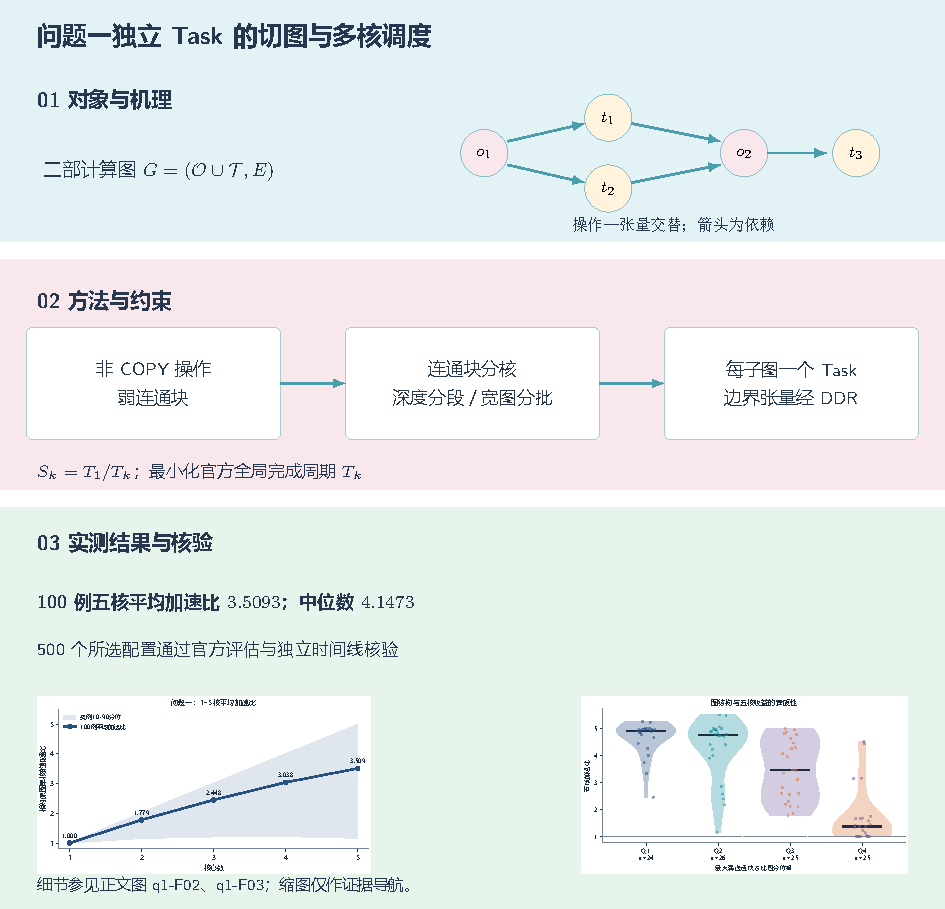
\includegraphics[width=160mm]{../求解/综合图/q1-overview.pdf}
\caption{问题一求解与核验总览}\label{fig:q1-overview}
\end{figure}
\FloatBarrier


多资源列表调度研究把核心、缓存、内存和I/O与任务先后约束共同纳入完工时间目标\cite{perotin2021}；针对有向无环任务图的HEFT算法还把执行代价和通信代价共同用于任务排序\cite{topcuoglu2002}。Kernighan--Lin以给定规模限制下的割边代价为划分目标\cite{kernighan1970}；多层次方法则通过粗化、粗图划分和细化逐步改善割边\cite{karypis1998}。本题同时存在Task切换、私有存储和共享DDR竞争，因此这些算法在本文作为建模参照，最终分数仍由题定评估器给出。

\subsection{切图与调度模型}

记输入二部图为 $G$，并写成 $G=(\mathcal{O}\cup\mathcal{T},E)$。$\mathcal{O}$ 是操作节点集合，$\mathcal{T}$ 是张量节点集合，$E$ 仅连接不同类型节点。对每个非 COPY 操作 $i$ 定义子图编号 $g(i)$；对子图 $g$ 定义核心编号 $a(g)$，并令每核子图序列形成一个全排列。所有非 COPY 操作必须且只能出现一次，子图依赖收缩图必须无环，同核序列须与该图的偏序相容。这些是硬约束，并在正式计分前由题目提供的校验程序执行。

对核数 $k$，令官方评估程序得到的全局完成时间为 $T_k$，原始整图单核完成时间为 $T_1$，则本题要求的加速比 $S_k$ 为
\begin{equation}\label{eq:q1-speedup}
S_k=\frac{T_1}{T_k},\qquad S_1=1.
\end{equation}
令 $D_k$ 为调度后 DDR 搬运字节数减去原图已有的搬运字节数。方案选择以最小化 $T_k$ 为第一目标；相同完成时间时，优先较小的 $D_k$。这里的 $T_k$ 是四条 Pipe、私有缓存、Task 等待与共享 DDR 带宽共同作用后的事件模拟结果，不用任何核内局部排布时间替代。

\subsection{候选构造与合法性}

采用连通块分核，先按官方图转换规则消去 COPY 端点，在非 COPY 操作上建立收缩依赖 DAG。该操作保留通过 COPY 链连接的先后关系。对其无向弱连通块，若两个操作落在不同块，就不存在块间非 COPY 依赖。连通块因此可以独立分核；块内部保持完整，避免直接切断其依赖。设块 $C$ 的粗负载为
\begin{equation}\label{eq:q1-load}
w(C)=\sum_{i\in C}(c_i+1),
\end{equation}
其中 $c_i$ 为题定计算周期。按 $w(C)$ 递减排序，把下一个块分给当前累计负载最小的核心；平局按核心编号固定。这是确定性的最长处理时间优先装箱。若把同核全部块合成一个子图，场景 A 只有每个活跃核心一个 Task，切换等待最少。该权重只负责生成候选，最终时间仍须由官方评估得出。

当一块过大时，仅保留整块可能让许多操作集中在一个核心。第二类候选先计算每个操作的最长前驱链深度 $d(i)$，再按深度划分最多八个相邻区段。在同一区段内求弱连通块并分核：以该区段的累计负载为主，给已有前驱所在核心一个有限的亲和奖励，防止为局部复用牺牲明显的负载均衡。每个“区段—核心”组合形成一个子图，同核按区段顺序执行。区段内不同块之间没有依赖，跨区段边只会从低深度指向高深度，故子图依赖图仍无环。分段可能新增边界搬运和 Task 等待，必须由实测决定是否采用。

对另一类极宽、但单个弱连通块较小的图，单核聚合会形成包含数千至上万操作的大 Task，也会显著增加参考核内调度程序的求解时间。规模规则使用输入图的操作数和最大块大小：若平均每核非 COPY 操作数超过 $2500$、最大块不超过 $600$ 个操作，则把已分配到同核的独立块顺序打包成目标至多 $800$ 操作的子图。所有块保持完整，同核批次依固定编号排序；这是改进算法生成与评估可行性的候选，并可能增加场景 A 的切换次数。较大块或不满足阈值时保留前两类候选。阈值在正式比较前固定，不根据某个测试结果倒调。

三类构造的图转换与连通块扫描均基于图的节点和边；排序主要增加块数的对数因子。实际总耗时还包括官方核内排布和全局模拟，因此单凭构造复杂度无法代表完整评估成本。每个候选先做覆盖、编号唯一、收缩无环及同核偏序检查，再交给官方场景 A 评估器。若候选触发内存不足或执行失败，则记录失败而不以缺失分数参与选择。所有正式结果保留原方案、原始官方响应与独立时间线复核。

\subsection{官方算例结果与分析}

正式计算覆盖100个官方算例、1至5核。每一配置对可用的连通块、八段与分批候选分别调用未修改的官方场景A评估器；候选通过合法性校验后按全局完成时间选择。图~\ref{fig:q1-f01}先显示输入图操作数与最大连通块占比的联合分布，说明这些算例既有整体性强的图，也有可独立分配的多块图。图~\ref{fig:q1-f02}按题目要求给出逐例求比再对100例取平均的1至5核加速比折线；淡色带为案例第10至第90百分位，不是均值置信区间。五核平均加速比为3.5093（无量纲），中位数为$4.1473$，第10与第90百分位分别为$1.1598$与$4.9885$。这说明多数图可利用多个核心，但接近单核的尾部算例依然存在；只报平均值会掩盖这一结构差异。

\begin{figure}[htbp]\centering
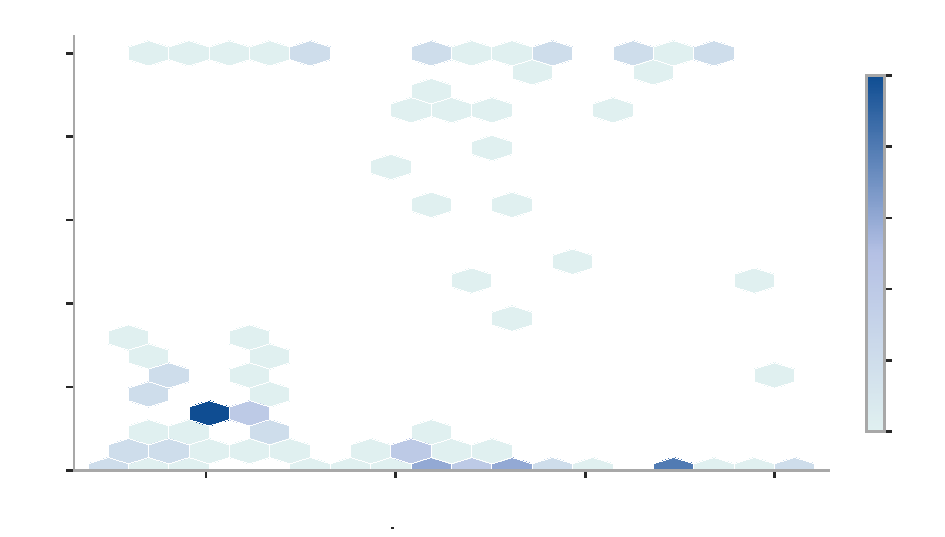
\includegraphics[width=160mm]{../求解/正式图件/q1-F01.pdf}
\caption{官方计算图结构分布}\label{fig:q1-f01}
\end{figure}

\begin{figure}[htbp]\centering
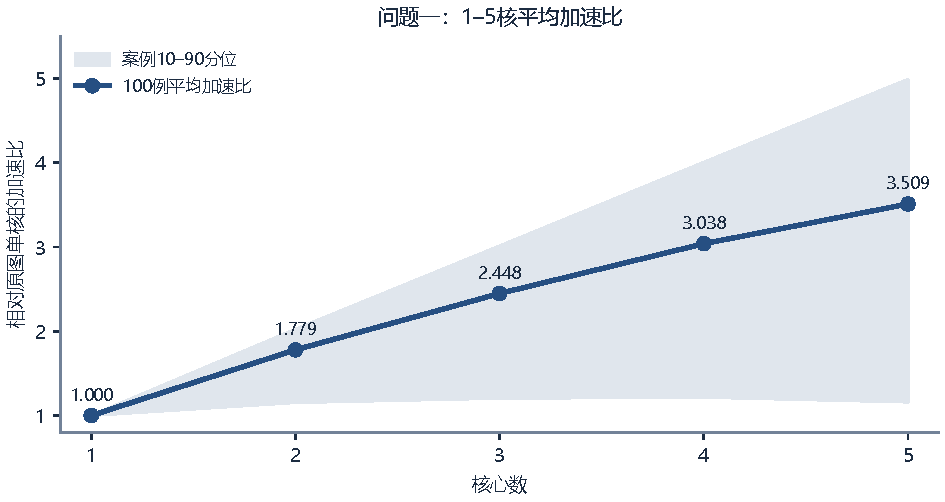
\includegraphics[width=160mm]{../求解/正式图件/q1-F02.pdf}
\caption{问题一核数扩展的平均加速比}\label{fig:q1-f02}
\end{figure}

各核数的平均加速比分别为$1.0000,1.7789,2.4477,3.0384,3.5093$。其增量递减，既反映并行工作被逐步分尽，也反映共享DDR、边界COPY与固定等待无法按核心数同比缩短。图~\ref{fig:q1-f03}把案例分层，使宽图与单块占优图的表现不被混为一种平均规律。逐例检查还发现26个算例在某一步增核后加速比下降，故不能把核数增加视作逐例单调改进；这些方案没有违反校验规则，而是完整事件模拟中的搬运、切换和调度次序共同变化。

\begin{figure}[htbp]\centering
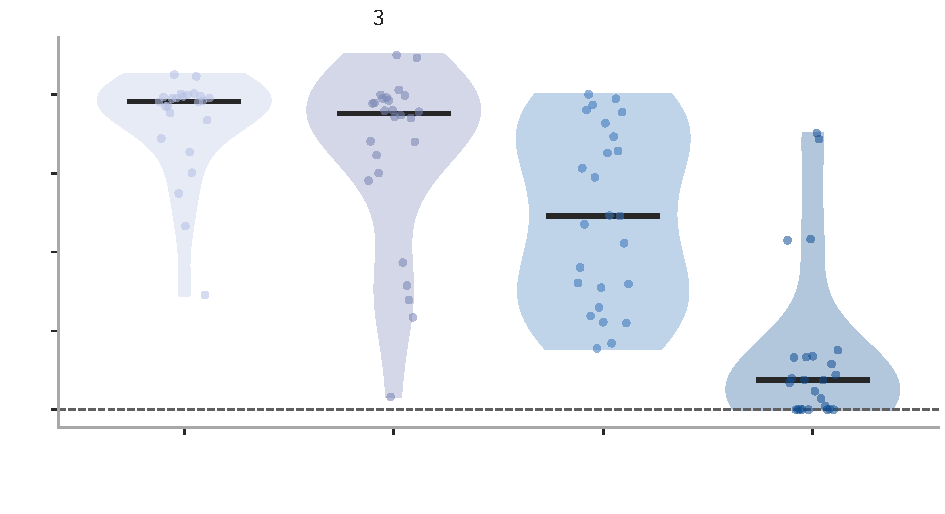
\includegraphics[width=160mm]{../求解/正式图件/q1-F03.pdf}
\caption{图结构分层与加速}\label{fig:q1-f03}
\end{figure}

五核最优候选的选择频数为连通块70例、深度分段22例、分批8例。连通块占多数，说明在这些输入中保持依赖块完整、减少跨子图搬运通常有利；但另30例需要对并行度或大Task求解成本作出折衷。图~\ref{fig:q1-f04}对照五核加速比与新增DDR搬运，并以操作数编码输入规模；零新增搬运落在轴原点。图~\ref{fig:q1-f05}将最大连通块大小和占比分箱，显示深度分段候选胜出的实际频率与每格样本数。两图共同约束“切得越细越好”的直觉：收益必须与新增传输和同步一起解释，不能把任一代理量当作官方目标。

\begin{figure}[htbp]\centering
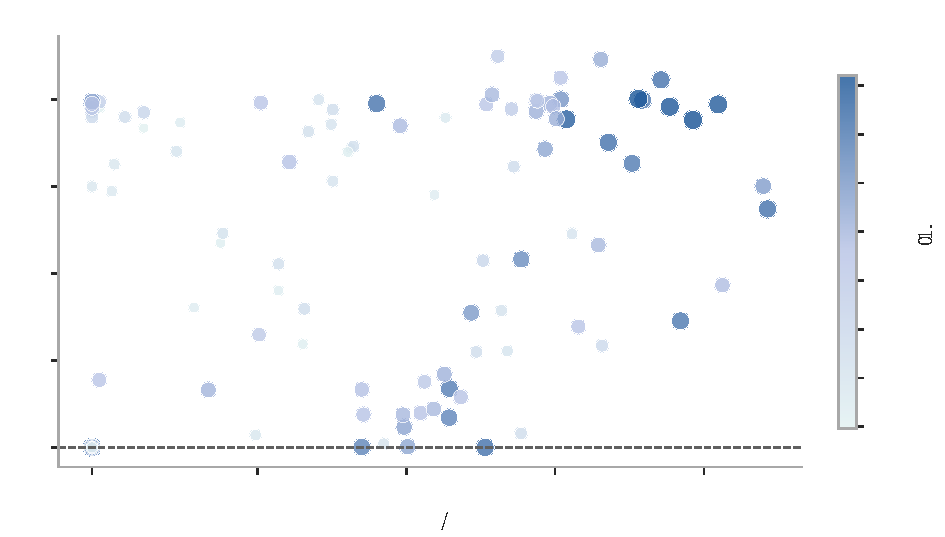
\includegraphics[width=160mm]{../求解/正式图件/q1-F04.pdf}
\caption{并行收益与新增搬运}\label{fig:q1-f04}
\end{figure}

\begin{figure}[htbp]\centering
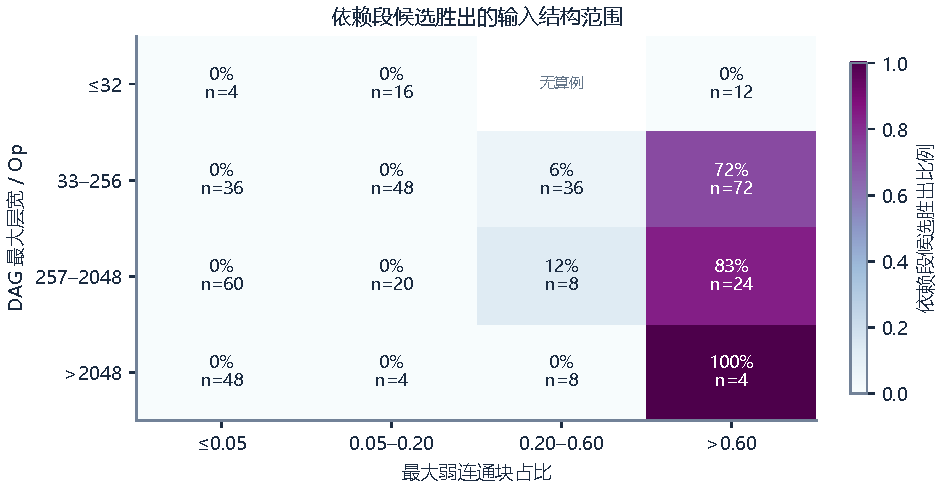
\includegraphics[width=160mm]{../求解/正式图件/q1-F05.pdf}
\caption{结构分箱中的候选胜率}\label{fig:q1-f05}
\end{figure}

最后，图~\ref{fig:q1-f06}报告候选评估的实际运行耗时与该候选相对同配置最佳完成时间的比。横轴是官方评估器处理候选的墙钟耗时，而不是所生成方案在处理器上的完成周期，也不含完整候选生成时间；因此只用来说明搜索预算与候选质量的折衷，不能作为题目加速比的分母。

\begin{figure}[htbp]\centering
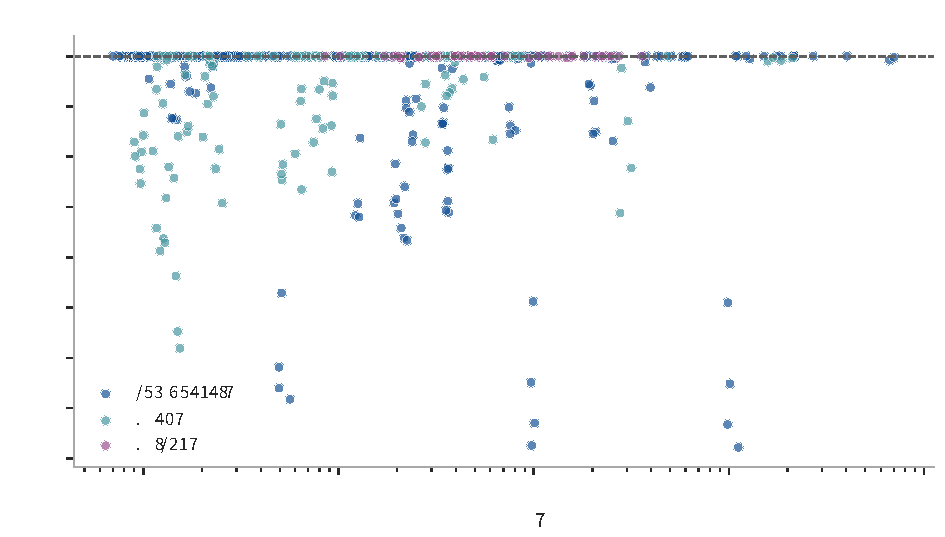
\includegraphics[width=160mm]{../求解/正式图件/q1-F06.pdf}
\caption{候选评估时间与规模}\label{fig:q1-f06}
\end{figure}

% Generated model comparison; edit scientific report and rerun the builder.
\noindent 本问是有显式约束和官方仿真目标的计算图组合优化；100 个图不提供最优方案标签，直接评价候选方案可复核，学习模型没有可验证的训练目标。\par


\subsection{结构分层的候选适配证据}

仅用总体五核均值无法检验候选构造是否符合图结构。为此令 $f$ 为最大弱连通块中的非 COPY 操作数占全部非 COPY 操作数的比例，按预先给定的四个范围对正式100例作互斥分层。表~\ref{tab:q1-structure-deep}从同一逐例记录重算各层的五核平均加速比、收缩 DAG 深度中位数与胜出候选频数；一个案例只计入一层。这里的深度是边数意义下的最长前驱层号，不是设备周期，不能直接与完成时间相减。四层样本量分别为38、21、13和28，因而表中的均值不是同样精度的总体估计，尤其不能把分层差异解释成随机试验中的处理效应。

\begin{table}[htbp]\centering
\caption{五核最大弱连通块占比分层的方案与收益}\label{tab:q1-structure-deep}
\small\begin{tabular}{lrrrrr}\toprule
最大块占比 $f$ & 算例数 & 平均加速比 & DAG深度中位数 & 连通块 & 分段/分批 \\ \midrule
$f\leq0.05$ & 38 & 4.6200 & 18.5 & 30 & 0/8 \\
$0.05<f\leq0.20$ & 21 & 3.8113 & 37.0 & 21 & 0/0 \\
$0.20<f\leq0.60$ & 13 & 3.6504 & 102.0 & 11 & 2/0 \\
$f>0.60$ & 28 & 1.7098 & 211.5 & 8 & 20/0 \\
\bottomrule\end{tabular}\end{table}
\begin{table}[htbp]\centering
\caption{问题一相邻核数下降的真实配置次数}\label{tab:q1-nonmonotone-deep}
\small\begin{tabular}{lrrr}\toprule
核数变化 & 加速比下降配置 & 同时换候选族 & 同时新增搬运增加 \\ \midrule
1→2 & 0 & 0 & 0 \\
2→3 & 7 & 0 & 7 \\
3→4 & 12 & 0 & 11 \\
4→5 & 22 & 1 & 19 \\
\bottomrule\end{tabular}\end{table}


最大块占比不超过$0.05$的38例，五核平均加速比为$4.6200$；其中30例由整块分配胜出，8例由分批候选胜出，深度中位数仅$18.5$。这组图的独立块多，分核时通常不必切断大型依赖块，所以低边界搬运与负载均衡可以同时实现。相反，在$f>0.60$的28例中，平均加速比为$1.7098$，深度中位数为$211.5$；20例需要深度分段，只有8例保持整块候选。该表给出构造策略与图结构相吻合的实测证据：块占比高时仅以整块为不可分单元，容易留下过大的串行片段。但分段胜出不等于高占比导致低收益的因果证明，因为最大块占比、DAG深度、操作周期、张量体积与带宽需求都随案例一起变化。

中间两个范围也有独立价值。$0.05<f\leq0.20$的21例全部选择连通块，均值$3.8113$；$0.20<f\leq0.60$的13例中只有2例改选分段，均值$3.6504$。这表明分段不是“块稍大便启用”的静态开关。其额外并行机会必须足以抵销 Task 等待和新增 DDR 搬运，最终仍以官方全局时间决定。表中把胜出频数与深度一起列出，也避免仅从图~\ref{fig:q1-f03}的分布形状推断具体哪个候选胜出。本文没有在分层后回改$2500$、$600$或$800$等构造阈值；这些数值固定于候选生成，分层表只是事后解释结果。

\subsection{结构代理量的反例检验}

分层均值显示趋势，但只有逐例反查才能判断最大块占比能否作为单独的决策规则。表~\ref{tab:q1-counterexamples}特意选取两例“小最大块但收益低”和两例“整图为单块但收益高”的正式五核结果。四例都来自原始100例，没有重新抽样或改变官方配置；其操作数、深度、最大层宽、搬运量和实际胜出候选均由同一逐例记录读取。这里的“收益低、高”是相对于同层总体趋势的描述，表中没有把案例从统计样本剔除。

\begin{table}[htbp]\centering
\caption{最大块占比不能单独预测五核收益的四例}\label{tab:q1-counterexamples}
\small\begin{tabular}{crrrrrc}\toprule
算例 & 最大块占比 & DAG深度 & 最大层宽 & 新增搬运/MiB & 加速比 & 胜出族 \\ \midrule
083 & 0.0323 & 125 & 31 & 14.36 & 2.3911 & 连通块 \\
092 & 0.0070 & 125 & 142 & 69.70 & 2.4555 & 分批 \\
062 & 1.0000 & 29 & 2181 & 22.83 & 4.5093 & 分段 \\
063 & 1.0000 & 27 & 817 & 8.57 & 4.4328 & 分段 \\
\bottomrule\end{tabular}\end{table}


算例083的最大块只占$0.0323$，却仅有$2.3911$倍五核加速；其DAG深度为125、最大层宽31，新增搬运约$14.36$ MiB。算例092的最大块占比更低，仅$0.0070$，但胜出的是分批候选，新增搬运约$69.70$ MiB，加速比$2.4555$。这两例说明“小块多”只表达可分配单元丰富，不说明张量边界便宜，也不说明所有可并行块会在资源争用下同时完成。尤其分批候选可能为降低超大Task的官方排布开销而被选中，其最终搬运代价必须一并报告。

反向的算例062与063最大块占比都是1，也即非COPY操作处于一个弱连通块，却分别达到$4.5093$和$4.4328$倍。两图的最大同层宽度分别为2181和817，远高于其深度29和27，深度分段能从同一个连接块中提出有用的并行片段。与算例016那种深度很长且宽度仅12的单块图相比，单块身份并不能确定可并行性。最大块占比衡量的是连通性，DAG深度和宽度衡量依赖方向上的并行机会，边界张量大小则决定让这些机会落在多核上要付出的传输成本。三个维度没有一个可以替代全局事件评估，但联合查看能解释为什么同一候选规则在不同图上产生不同效果。

这个反例检验也给下一轮候选设计指出具体方向：对占比高且宽度大的图，应尝试围绕依赖层内的可交换操作划分，同时限制边界张量总量；对占比低但COPY仍大的图，则应检查许多小块是否共享同一张量输入、是否被调度到过多不同核心。上述策略尚未成为本次正式结果，本文不把它们写成已验证算法或成绩。当前提交方案只使用前述三个已经逐例合法评估的候选族。

\subsection{合法性与离散事件目标的连接}

切图候选之所以可用于正式比较，首先依赖结构上的封闭性。令消去 COPY 端点后的非 COPY 依赖 DAG 为 $G'=(V',E')$，弱连通块集合为 $\mathcal C$。每个 $v\in V'$ 属于且仅属于一个弱连通块；若一条边 $(u,v)\in E'$ 的两个端点处于不同块，这两个块本应由该边连接，与弱连通定义矛盾。因此整块分核时，块间没有遗漏的原图依赖；同核多个块的固定排列只附加执行顺序，不会删除一条先后约束。每个操作恰好被指派一次，故块到核心、核心到子图的映射同时满足唯一覆盖和编号完备。

深度分段候选另令 $d(v)$ 为从任一源点到 $v$ 的最长依赖路径边数。对每条依赖边 $(u,v)$ 有 $d(v)\geq d(u)+1$。把有序深度轴切成相邻区段后，跨区段边只能由早段指向晚段；同一区段内再按弱连通块分割，区段内部不同块之间不存在依赖边。于是以“区段、核心”为子图并按区段序编号时，任何收缩后的边都不可能由晚段回到早段，也不可能形成区段内的块间环。该推导解释了候选构造的合法性来源，但不证明所选方案时间最短；具体容量约束和所有细节仍交给官方校验器与独立时间线检查。

全局 Makespan 是所有核心、Pipe 和共享资源上的事件最终完成时刻，可以写为 $T=\max_e t_e^{\mathrm{finish}}$。它一般不等于各核计算周期之和，也不等于简单的“最长链计算量加总搬运量”：COPY可能与计算重叠，多个核心的DDR请求又会竞争同一带宽池，固定 Task 等待也会改变后续事件次序。因此粗负载$w(C)$只在候选生成时平衡工作量，不作为正式目标的近似分数；深度$d(v)$只保证依赖方向，不代表纳入资源争用后的关键路径。本文的最终选择规则是在同一图、同一核数下对实际成功通过官方评估的候选取最小$T$，其保证仅相对于这组已评估候选成立。没有对所有合法切图与同核排序枚举，不能声称全局最优或给出未经证明的最优性缺口。

\subsection{增核非单调性与稳健性边界}

逐例核数曲线提供了均值曲线之外的反例。表~\ref{tab:q1-nonmonotone-deep}把四次相邻核数变化分别统计：从一核到两核没有下降配置；二到三、三到四、四到五核分别有7、12、22个下降配置。四列相加为41次“案例—核数转移”，涉及26个不同案例，不能把41误写成41个图。下降转移中仅1次同时更换了候选族，而37次伴随新增搬运量上升；后一个并发关系支持继续检查跨核张量，但不构成搬运单独造成下降的因果识别。同一候选族在两个核数下仍可能产生不同的块分配和Task顺序，故“候选族没变”也不是严格固定方案的反事实。

该现象决定了提交策略应保留每个要求核数的独立方案，而不是把五核的划分机械删核后视作二至四核答案。对图结构极宽的案例，额外核心可利用互不依赖的块；对长链或高边界流量案例，增加核心会使同步与COPY的相对成本上升。仅当候选在该核数经过合法性检查、官方全局评估并完成结果核验后，其时间才进入该核数的逐例成绩。表~\ref{tab:q1-nonmonotone-deep}同时限定了本文的稳健性主张：平均收益随核数增加，并不意味着100条个体曲线逐条单调；后续改进应把“新增核是否真正释放可并行依赖”纳入候选筛选，而不改变官方评价口径。

\subsection{结果核验与本问结论}

逐例结构诊断给出了均值无法表达的两端。算例016有$17995$个非COPY操作，全部属于同一弱连通块；其收缩DAG深度为$2441$、最大同层宽度仅$12$，五核候选仍选整块方案，完成周期$7715523$，相对原始单核的加速比恰为$1$。这个实例表明，核数可用并不意味着存在足够的独立块可直接分配。相反，算例059仅有$2752$个非COPY操作却分成$64$个弱连通块，最大块占比$0.015625$，五核整块分配后的完成周期为$150782$，加速比达到$5.5011$。它超过理想线性值$5$并非计时错误：本题基准是原始整图的官方单核时间，改变切图后也会改变核内排布及开销。因此不能把$k$误当成每个方案的严格加速上界。

两例都选连通块候选，但形成截然不同的响应，说明“胜出候选族”不足以描述方案质量。弱连通块数、关键路径深度和同层宽度必须与实际完成时间并读；即使图结构提示并行机会，也只能把它当作筛选候选的依据，不能跳过Task等待、COPY和共享带宽的官方评估。图~\ref{fig:q1-f03}的宽分布及图~\ref{fig:q1-f04}的成本散点正是对此逐例差异的总体检验。

每个最终方案均重新进行操作唯一覆盖、核心编号、无环和同核序列偏序核验，并保留官方原始响应与逐例方案。独立收集程序复算$T_1/T_k$、核对报告中的完成周期和新增搬运字段，再用事件时间线检查完成时刻；独立重算后，所选五百组方案的覆盖、时间线及官方响应交叉核验全部通过。此复核在官方评估器之外运行，避免把一次成功返回当成充分正确性证明。

本问方法保留三个有限、事先定义的候选族，没有枚举所有合法切图，故结果是可复核的可行调度而非全局最优性证明。尤其在大弱连通块内，深度分段最多八层，可能错过更细的依赖划分；而负载权重$w(C)$未显式预测共享带宽拥塞。图~\ref{fig:q1-f03}的低加速尾部提示后续应针对依赖关键路径和边界张量位置继续设计候选，但任何新策略仍需在同一官方评估链中成对比较。






